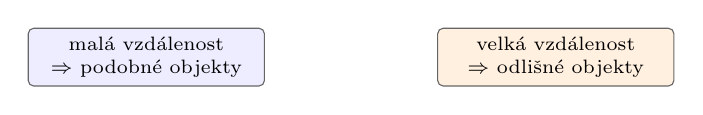
\begin{tikzpicture}[
    box/.style={
        draw=black!60,
        rounded corners=2pt,
        minimum width=3cm,
        minimum height=0.72cm,
        align=center,
        font=\scriptsize
    }
]
    \node[box, fill=blue!7] at (-2.6,0)
        {malá vzdálenost\\$\Rightarrow$ podobné objekty};

    \node[box, fill=orange!12] at (2.6,0)
        {velká vzdálenost\\$\Rightarrow$ odlišné objekty};
\end{tikzpicture}
